\documentclass[12pt]{article}

% ---------- Page layout & fonts ----------
\usepackage[margin=1in]{geometry}
\usepackage[T1]{fontenc}
\usepackage{lmodern}
\usepackage{microtype}            % better spacing/justification
\usepackage{enumitem}             % customizable lists
\usepackage{xcolor}

% ---------- Math ----------
\usepackage{amsmath}
\usepackage{amssymb}              % \mathbb, extra symbols
\usepackage{amsthm}               % theorem environments
\usepackage{mathtools}            % amsmath extensions
\usepackage{bm}                   % bold math: \bm{\theta}
\usepackage{braket}               % Dirac notation: \ket{0}, \bra{\psi}, \braket{\phi|\psi}
\setcounter{MaxMatrixCols}{16}    % allow the 16-column four-qubit matrix below
\numberwithin{equation}{section}  % equations numbered as <section>.<n>

% ---------- Figures, tables, circuits ----------
\usepackage{graphicx}
\usepackage{float}                % [H] placement
\usepackage{caption}
\usepackage{subcaption}           % side-by-side subfigures
\usepackage{booktabs}             % \toprule, \midrule, \bottomrule
\usepackage{tabularx}
\usepackage{multirow}
\usepackage{tikz}
\usepackage{quantikz}             % quantum circuit diagrams

% ---------- Algorithms & code ----------
\usepackage{algorithm}
\usepackage{algpseudocode}
\usepackage{listings}             % code blocks (e.g. Python/PennyLane)
\lstset{basicstyle=\ttfamily\small, breaklines=true, frame=single,
        keywordstyle=\color{blue}, commentstyle=\color{gray}}

% ---------- Units ----------
\usepackage{siunitx}

% ---------- References (load last) ----------
\usepackage[colorlinks=true, linkcolor=blue, citecolor=blue, urlcolor=blue]{hyperref}
\usepackage[capitalise, nameinlink]{cleveref}  % \cref{eq:rx} -> "Equation (3.1)"

% ---------- Theorem environments ----------
\theoremstyle{definition}
\newtheorem{definition}{Definition}[section]
\theoremstyle{plain}
\newtheorem{theorem}{Theorem}[section]
\newtheorem{lemma}[theorem]{Lemma}
\newtheorem{proposition}[theorem]{Proposition}
\theoremstyle{remark}
\newtheorem{remark}{Remark}[section]

% Edit these two lines to customize the title page.
\newcommand{\DocumentTitle}{Quantum Neural Networks}
\newcommand{\DocumentSubtitle}{Theory, Architectures, and Applications}

\begin{document}

\begin{titlepage}
    \centering
    \vspace*{0.30\textheight}

    {\Huge\bfseries
        \DocumentTitle
    \par}

    \vspace{1.25em}

    {\Large\color{gray}
        \DocumentSubtitle
    \par}

    \vfill
\end{titlepage}

\section{Background}
Classical machine learning has gained huge success in recent years especially deep learning models such as multi-layer perceptrons (MLP), Convolution Neural Networks (CNN), Recurrent Neural Netowrks (RNN), Transformers, and Graph Neural Netowrks (GNN). These architectures, due to its inductive bias and with development of hardware accelerators, have been applied in many fieds such as image processing, audio-speech processing, language modeling, and fraud detection. However, as the models are getting larger and larger, the computing power required is also growing exponentially. Governments and private companies are spending billions of dollar on building data center to satisfy the compute needs of now. 

On the other hand, a new paradigm of computing started to shine on the stage -- quantum computing. 

\section{Classical Neural Networks}


\section{Quantum Neural Networks}

\subsection{Basics of Quantum Computing}
If we have multiple qubits, let's say $N$ qubits. Each qubit, individually is operated by a quantum gate $U_1,U_2,\cdots,U_N$. Then the operation matrix on the entire quantum state is
\[U=U_1\otimes U_2\otimes U_3\otimes \cdots \otimes U_N\]

CNOT gate is an interesting gate that takes 2 qubits as input. Its main purpose is to produce conditional independence between these 2 qubits. In these 2 qubits, one is target and the other is control. The logic is:
\[\ket{c,t}\xrightarrow{\text{CNOT}}\ket{c,t\oplus c}\]
That is flipping the target qubit if the control qubit is 1, otherwise do nothing. For example, if we let $q_0$ be the target and $q_1$ be the control and we use little-endian format $\ket{q_1q_0}$. 
\[\begin{aligned}
    \ket{00}\rightarrow\ket{00}\\
    \ket{01}\rightarrow\ket{01}\\
    \ket{10}\rightarrow\ket{11}\\
    \ket{11}\rightarrow\ket{10}
\end{aligned}\]
The operation matrix of CNOT gate is therefore:
\[CNOT_{q_1\rightarrow q_0}=\begin{bmatrix}
    1&0&0&0\\0&1&0&0\\0&0&0&1\\0&0&1&0
\end{bmatrix}\]
For example,
\[CNOT_{q_1\rightarrow q_0}\ket{10}=\begin{bmatrix}1&0&0&0\\0&1&0&0\\0&0&0&1\\0&0&1&0\end{bmatrix}\begin{bmatrix}0\\0\\1\\0\end{bmatrix}
=\begin{bmatrix}0\\0\\0\\1\end{bmatrix}=\ket{11}\]
Please be aware that if $q_0$ is the control and $q_1$ is the target, then
\[CNOT_{q_0\rightarrow q_1}=\begin{bmatrix}
    1&0&0&0\\0&0&0&1\\0&0&1&0\\0&1&0&0
\end{bmatrix}\]
For example, 
\begin{equation*}
    CNOT_{q_0\rightarrow q_1}\ket{01}=\begin{bmatrix}
    1&0&0&0\\0&0&0&1\\0&0&1&0\\0&1&0&0\end{bmatrix}\times\begin{bmatrix}0\\1\\0\\0\end{bmatrix}=
    \begin{bmatrix}0\\0\\0\\1\end{bmatrix}=\ket{11}
\end{equation*}

Then, how is entanglment produced using CNOT gate? In Figure~\ref{fig:bellstate}, we have two qubits, both in $\ket{0}$ as initial state. Then, one of them undergo Hadmard operation, which makes the state become:
\[\ket{\psi}=\frac{1}{\sqrt{2}}(\ket{00}+\ket{01})\]
After applying a CNOT gate on these 2 qubits, we have:
\[CNOT_{q_0\rightarrow q_1}\ket{\psi}=\frac{1}{\sqrt{2}}(\ket{00}+\ket{11})\]
Now, these 2 qubits are entangled! This means that if we know the state of one of the qubits, we immediately know the state of the other without measuring it. \\
\begin{figure}[htbp]
    \centering
    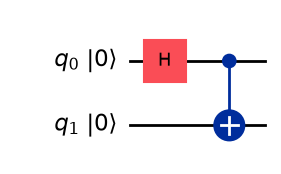
\includegraphics[width=0.5\textwidth]{figures/bell.png}
    \caption[short]{How entanglment is produced in bell state}
    \label{fig:bellstate}
\end{figure}
\textbf{Rule of thumb.} For a two-qubit syste:
\[\ket{\psi_1\psi_0}=a\ket{00}+b\ket{01}+c\ket{10}+\ket{11}\]
The quickest way to check if these two qubits are entangled is:
\begin{equation}
    \begin{cases}
        ad-bc\neq 0, \quad \text{entangled}\\
        ad-bc=0, \quad \text{product state/non-entangled}
    \end{cases}
    \label{eq:entangle}
\end{equation}

\subsection{Dissection of QNN}
Similar to classical neural networks, quantum neural networks (QNN) also tries to universally approximate functions but in a foundamental different way. Figure~\ref{fig:qnn} shows a \textbf{3-qubit} circuit architecture of a standard quantum neural networks. Simply speaking, it is composed of layers of rotation gate (X,Y,Z) and CNOT gate. In the end, the each wire has a measurement gate (usually Z-basis). 
\begin{figure}[htbp]
\centering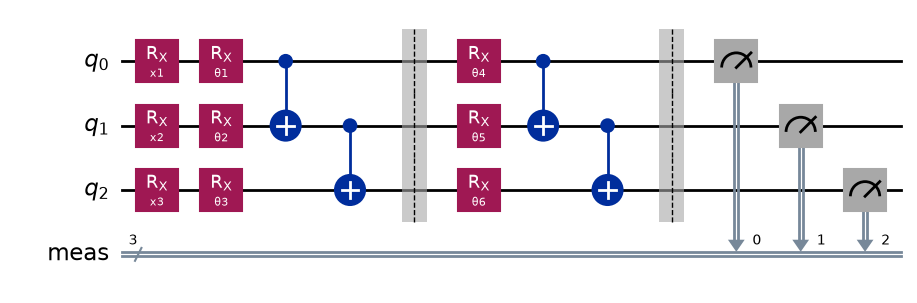
\includegraphics[width=0.8\textwidth]{figures/qnn_3.png}
\caption[short]{A standard quantum neural network}
\label{fig:qnn}    
\end{figure}
Let's look at each gate one by one. Firstly, there are three types of rotation gate $R_x,R_y,R_z$. Any single-qubit gate is a $2\times2$ unitary matrix and these three matrices, variants of Pauli-matrices, rotates the vector in the bloch sphere about $x,y,z$ axis by $\theta$ degrees. Their mathmatical definition is as follows:

\begin{equation}
    R_x(\theta)\equiv e^{-i\theta X/2}=\cos(\frac{\theta}{2})I-i\sin(\frac{\theta}{2})X=\begin{bmatrix}
    \cos(\frac{\theta}{2})&-i\sin(\frac{\theta}{2})\\-i\sin(\frac{\theta}{2})&\cos(\frac{\theta}{2})
\end{bmatrix}.
\end{equation}
\begin{equation}
    R_y(\theta)\equiv e^{-i\theta Y/2}=\cos(\frac{\theta}{2})I-i\sin(\frac{\theta}{2})Y=\begin{bmatrix}
    \cos(\frac{\theta}{2})&-\sin(\frac{\theta}{2})\\ \sin(\frac{\theta}{2})&\cos(\frac{\theta}{2})
\end{bmatrix}.
\end{equation}
\begin{equation}
    R_z(\theta)\equiv e^{-i\theta Z/2}=\cos(\frac{\theta}{2})I-i\sin(\frac{\theta}{2})Z=\begin{bmatrix}
    e^{-i\theta/2}&0\\0&e^{i\theta/2}
\end{bmatrix}.
\end{equation}
Controlled-NOT (CNOT) gate has two input qubits, known as control qubit and target qubit, respectively. In terms of the computational basis, the action of CNOT is given by $\ket{c}\ket{t}\rightarrow\ket{c}\ket{t\oplus c}$. That is if the control qubit is set to $\ket{1}$ then the target qubit is flipped, otherwise the target qubit is left alone. Thus, in the computational basis $\ket{contro,target}$ the matrix representation of CNOT is:
\[\begin{bmatrix}
    1&0&0&0\\0&0&0&1\\0&0&1&0\\0&1&0&0
\end{bmatrix}.\]
For example, if a two-qubit system is in state $\ket{11}$, which in basis vector is $\begin{bmatrix}0\\0\\0\\1\end{bmatrix}$. Here we follow little-endian (LSB)convention ($\ket{q_1q_0}$) and let $\ket{q_0}$ be the control qubit and $\ket{q_1}$ be the target qubit. When a CNOT gate is applied to it:
\[\begin{bmatrix}1&0&0&0\\0&0&0&1\\0&0&1&0\\0&1&0&0\end{bmatrix}\times
\begin{bmatrix}0\\0\\0\\1\end{bmatrix}=\begin{bmatrix}0\\1\\0\\0\end{bmatrix}=\ket{01}\]
\[CNOT\ket{11}\rightarrow\ket{01}\]
These three rotation gates and CNOT gate are also known universal gates in quantum computer, similar to NOR and NAND in classical computer. Any unitary matrix can be decomposed to sequenec of rotation gates and CNOT gate. Similar to classical neural network, quantum neural network also has input, hidden and output layers, which corresponds to encoding, rotation and entanglment in Hilbert Space, and measurement. Let's look at them one by one.

\subsection{Input Layer: Encoding}
For most of machine learning tasks, the data is classical. Therefore, we need a way to encode the classical data into quantum states. Three main encoding approaches are:
\begin{enumerate}
    \item \textbf{Amplitude Encoding}
    \item \textbf{Basis Encoding}
    \item \textbf{Angular Encoding}
\end{enumerate}
Of course, there are other more advanced encoding such as Pauli Encoding and IQP Encoding but it's not in the scope of this article. Here, we first talk about the most common encoding method - \textbf{Angular Encoding} because it's the easiest to prepare from engineering perspective. Just as the name suggests, the classical data $x_i$ is mapped into a rotation angle using rotation gates. Figure~\ref{fig:encode} shows how a 3-dimension input vector is embedded into a quantum circuit. Each qubit, represented by a single line here, starts with 0 basis state $\ket{0}$. Then qubit is followed by a rotation gate (can be $R_x,R_y,R_z$). These rotation gates will then be parametrized by the input values $x_1,x_2,x_3$. For example, for the first qubit (little-endian), the starting state is $\ket{0}=\begin{bmatrix}1\\0\end{bmatrix}$. Then the rotation gate, let's say $R_x$, is parametrized by $x_1$:

\[R_x(x_1)=\begin{bmatrix}
    \cos(\frac{x_1}{2})&-i\sin(\frac{x_1}{2})\\-i\sin(\frac{x_1}{2})&\cos(\frac{x_1}{2})
\end{bmatrix}.\]
Then the qubit is operated as:
\[R_x(x_1)\ket{0}=
    \begin{bmatrix}
    \cos(\frac{x_1}{2})&-i\sin(\frac{x_1}{2})\\-i\sin(\frac{x_1}{2})&\cos(\frac{x_1}{2})\end{bmatrix}\times \begin{bmatrix}1\\0\end{bmatrix}=\begin{bmatrix}
    \cos(\frac{x_1}{2})\\-i\sin(\frac{x_1}{2})
    \end{bmatrix}\]
This is equivalent to:
\[\ket{0}\rightarrow \cos(\frac{x_1}{2})\ket{0}+(-i\sin(\frac{x_1}{2}))\ket{1}\]

If you use $R_y$, then you will have:
\[R_y(x_1)\ket{0}=
    \begin{bmatrix}
    \cos(\frac{x_1}{2})&-\sin(\frac{x_1}{2})\\\sin(\frac{x_1}{2})&\cos(\frac{x_1}{2})\end{bmatrix}\times \begin{bmatrix}1\\0\end{bmatrix}=\begin{bmatrix}
    \cos(\frac{x_1}{2})\\\sin(\frac{x_1}{2})
    \end{bmatrix}\]


Similarly, for the rest of input values $x_2,x_3,x_4$, the quantum states of the qubits become (assume we use $R_x$):
\[q_1(x_2)=\begin{bmatrix}\cos(\frac{x_2}{2})\\-i\sin(\frac{x_2}{2})\end{bmatrix},\quad
q_2(x_3)=\begin{bmatrix}\cos(\frac{x_3}{2})\\-i\sin(\frac{x_3}{2})\end{bmatrix}\]

\begin{figure}[htbp]
    \centering
    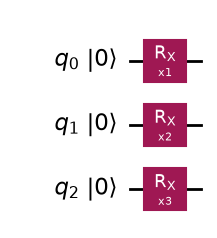
\includegraphics[width=0.2\textwidth]{figures/encode_3.png}
    \caption{Input layer of a QNN using angluar encoding.}
    \label{fig:encode}
\end{figure}

If we look at the 3-qubit system holistically, which is also known as product state, the state transitions from $\ket{000}$ to $\ket{q_2q_1q_0}$. Mathmatically as follows:
\begin{equation*}
\begin{bmatrix}
    1\\0\\0\\0\\0\\0\\0\\0
\end{bmatrix}\xrightarrow{\text{angle encoding}}
\begin{bmatrix}\cos(\frac{x_3}{2})\\-i\sin(\frac{x_3}{2})\end{bmatrix}\otimes
\begin{bmatrix}\cos(\frac{x_2}{2})\\-i\sin(\frac{x_2}{2})\end{bmatrix}\otimes
\begin{bmatrix}\cos(\frac{x_1}{2})\\-i\sin(\frac{x_1}{2})\end{bmatrix}    
\end{equation*}
This is equivalent to:
\begin{equation*}
\ket{q_2q_1q_0}=\ket{q_2}\otimes\ket{q_1}\otimes\ket{q_0}
\end{equation*}
The statevector of entire circuit can be rewritten into tensor product of statevector of each single qubit becuase entanglement has not yet formed. \\
The tensor product of three $2\times 1$ vectors is a $8\times 1$ vector, which is expanded as follows:
\begin{equation*}
\psi({x_3,x_2,x_1})= \begin{bmatrix}
\cos(\frac{x_3}{2})\cos(\frac{x_2}{2})\cos(\frac{x_1}{2})\\[6pt]
-i\cos(\frac{x_3}{2})\cos(\frac{x_2}{2})\sin(\frac{x_1}{2})\\[6pt]
-i\cos(\frac{x_3}{2})\sin(\frac{x_2}{2})\cos(\frac{x_1}{2})\\[6pt]
-\cos(\frac{x_3}{2})\sin(\frac{x_2}{2})\sin(\frac{x_1}{2})\\[6pt]
-i\sin(\frac{x_3}{2})\cos(\frac{x_2}{2})\cos(\frac{x_1}{2})\\[6pt]
-\sin(\frac{x_3}{2})\cos(\frac{x_2}{2})\sin(\frac{x_1}{2})\\[6pt]
-\sin(\frac{x_3}{2})\sin(\frac{x_2}{2})\cos(\frac{x_1}{2})\\[6pt]
i\sin(\frac{x_3}{2})\sin(\frac{x_2}{2})\sin(\frac{x_1}{2})
\end{bmatrix}    
\end{equation*}
If we look each qubit individually, the encoding is a $2\times 2$ matrix. However, if we look the encoding holistically on the entire 3 qubit system, it's a $2^3\times2^3=8\times 8$ matrix, which is also a tensor product of all three rotation matrices:
\begin{equation*}
\begin{bmatrix}\cos(\frac{x_3}{2})&-i\sin(\frac{x_3}{2})\\-i\sin(\frac{x_3}{2})&\cos(\frac{x_3}{2})\end{bmatrix}\otimes
\begin{bmatrix}\cos(\frac{x_2}{2})&-i\sin(\frac{x_2}{2})\\-i\sin(\frac{x_2}{2})&\cos(\frac{x_2}{2})\end{bmatrix}\otimes
\begin{bmatrix}\cos(\frac{x_1}{2})&-i\sin(\frac{x_1}{2})\\-i\sin(\frac{x_1}{2})&\cos(\frac{x_1}{2})\end{bmatrix}    
\end{equation*}

This makes sense becuase with 3 qubits, the quantum state is in $\mathbb{C}^2\otimes\mathbb{C}^2\otimes\mathbb{C}^2=\mathbb{C}^{8}$ and the operation shall also be a $8\times 8$ matrix as follows. To make it readable, let's define:
\[c_j=\cos\left(\frac{x_j}{2}\right),\qquad s_j=\sin\left(\frac{x_j}{2}\right),\qquad j=1,2,3,4.\]

\begin{equation*}
U = R_x(x_3)\otimes R_x(x_2)\otimes R_x(x_1)
\end{equation*}

The matrix is as follows:
\begin{equation}
\begin{bmatrix}
c_3c_2c_1 & -ic_3c_2s_1 & -ic_3s_2c_1 & -c_3s_2s_1 & -is_3c_2c_1 & -s_3c_2s_1 & -s_3s_2c_1 & is_3s_2s_1\\
-ic_3c_2s_1 & c_3c_2c_1 & -c_3s_2s_1 & -ic_3s_2c_1 & -s_3c_2s_1 & -is_3c_2c_1 & is_3s_2s_1 & -s_3s_2c_1\\
-ic_3s_2c_1 & -c_3s_2s_1 & c_3c_2c_1 & -ic_3c_2s_1 & -s_3s_2c_1 & is_3s_2s_1 & -is_3c_2c_1 & -s_3c_2s_1\\
-c_3s_2s_1 & -ic_3s_2c_1 & -ic_3c_2s_1 & c_3c_2c_1 & is_3s_2s_1 & -s_3s_2c_1 & -s_3c_2s_1 & -is_3c_2c_1\\
-is_3c_2c_1 & -s_3c_2s_1 & -s_3s_2c_1 & is_3s_2s_1 & c_3c_2c_1 & -ic_3c_2s_1 & -ic_3s_2c_1 & -c_3s_2s_1\\
-s_3c_2s_1 & -is_3c_2c_1 & is_3s_2s_1 & -s_3s_2c_1 & -ic_3c_2s_1 & c_3c_2c_1 & -c_3s_2s_1 & -ic_3s_2c_1\\
-s_3s_2c_1 & is_3s_2s_1 & -is_3c_2c_1 & -s_3c_2s_1 & -ic_3s_2c_1 & -c_3s_2s_1 & c_3c_2c_1 & -ic_3c_2s_1\\
is_3s_2s_1 & -s_3s_2c_1 & -s_3c_2s_1 & -is_3c_2c_1 & -c_3s_2s_1 & -ic_3s_2c_1 & -ic_3c_2s_1 & c_3c_2c_1
\end{bmatrix}
\label{eq:unitarymatrix}
\end{equation}
Please be aware that since we use little-endian convention, the tensor product of operation matrix follows the same order as the qubit. 
If our initial state is $\ket{0}$, then the resulting state is the first column of this matrix. In fact, the matrix is
\[U_{\mathbf{b,b'}}=(-i)^{d_H(\mathbf{b,b'})}\prod_{j:b_j=b'_j}c_j \prod_{j:b_j\neq b'_j}s_j\]
where $d_H(\mathbf{b,b'})$ is Hamming distance between target state and initial state. \\
Before concluding angle encoding, there is one more thing - \textbf{scaling}. As you might have observed, the trignometric functions are all periodic ($2\pi$) meaning that
\[\ket{\psi(x)}=\ket{\psi(x+2\pi)}\]
If the range of classical data is larger than $2\pi$, then two different classical values will be mapped to the same quantum state, causing information loss. Therefore, scaling must be conducted such that the input values, before encoding, must be between $0$ and $\pi$. This is becuase the periodicity of cosine and sine functions are $2\pi$, so the periodicity in $\cos(\frac{x}{2})$ is $\pi$. A simple and most common way to do scaling is as follows:
\[\theta=\pi\frac{x-x_{min}}{x_{max}-x_{min}}\]
Now, the features are mapped into a non-repeatitive and continuous angle space. Finally, there are many variants of angle encoding such as XYZ encoding, data-reuploading, multiscale, and adaptive encoding. What has to be aware of is that encoding can have notrivial impact on the representation capacity of the model. 

\subsection{Hidden Layer - Rotation}
Now, after angle encoding, each qubit is in the state 
\begin{equation*}
\ket{\psi}\cos(\frac{x_i}{2})\ket{0}+(-i\sin(\frac{x_i}{2}))\ket{1}=\begin{bmatrix}
\cos(\frac{x_1}{2})\\-i\sin(\frac{x_1}{2})\end{bmatrix}.
\end{equation*}
Then, this qubit will go through another rotation gate, let's say $R_x$, which is parametrized by $\theta$, resembling the weight in classical neural networks. The state becomes:

\[R_x(\theta)\ket{\psi}=\begin{bmatrix}\cos(\frac{\theta}{2})&-i\sin(\frac{\theta}{2})\\-i\sin(\frac{\theta}{2})&\cos(\frac{\theta}{2})\end{bmatrix}\times\begin{bmatrix}\cos(\frac{x_i}{2})\\-i\sin(\frac{x_i}{2})\end{bmatrix}=\begin{bmatrix}
\cos(\frac{\theta}{2})\cos(\frac{x_i}{2})-\sin(\frac{\theta}{2})\sin(\frac{x_i}{2})\\
-i\sin(\frac{\theta}{2})\cos(\frac{x_i}{2})-i\cos(\frac{\theta}{2})\sin(\frac{x_i}{2})
\end{bmatrix}\]


Using following trignometric identity, we can further simplify. 
\[\begin{aligned}
\cos(A+B)=\cos(A)\cos(B)-\sin(A)\sin(B)\\
\sin(A+B)=\sin(A)\cos(B)+\cos(A)\sin(B)
\end{aligned}\]

\[
\begin{bmatrix}
\cos(\frac{\theta}{2})\cos(\frac{x_i}{2})-\sin(\frac{\theta}{2})\sin(\frac{x_i}{2})\\
-i\sin(\frac{\theta}{2})\cos(\frac{x_i}{2})-i\cos(\frac{\theta}{2})\sin(\frac{x_i}{2})
\end{bmatrix}=\begin{bmatrix}\cos(\frac{\theta+x_i}{2})\\-i\sin(\frac{\theta+x_i}{2})\end{bmatrix}
\]
For example, in Figure~\ref{fig:hidden3_1}, the first qubit becomes: 
\begin{equation*}
\ket{q_0}=\begin{bmatrix}\cos(\frac{\theta_1+x_1}{2})\\-i\sin(\frac{\theta_1+x_1}{2})\end{bmatrix}.
\end{equation*}
For the rest of qubits, the states becomes:
\begin{equation*}
q_1=\begin{bmatrix}\cos(\frac{\theta_2+x_2}{2})\\-i\sin(\frac{\theta_2+x_2}{2})\end{bmatrix},\quad
q_2=\begin{bmatrix}\cos(\frac{\theta_3+x_3}{2})\\-i\sin(\frac{\theta_3+x_3}{2})\end{bmatrix}
\end{equation*}
The entire 3-qubit system then becomes the tensor product of these four vectors:
\begin{equation*}
\psi_{q_3q_2q_1}=
\begin{bmatrix}\cos(\frac{\theta_3+x_3}{2})\\-i\sin(\frac{\theta_3+x_3}{2})\end{bmatrix}\otimes
\begin{bmatrix}\cos(\frac{\theta_2+x_2}{2})\\-i\sin(\frac{\theta_2+x_2}{2})\end{bmatrix}\otimes
\begin{bmatrix}\cos(\frac{\theta_1+x_1}{2})\\-i\sin(\frac{\theta_1+x_1}{2})\end{bmatrix}   
\end{equation*}
Which can be expaned as:
\begin{equation}
\begin{bmatrix}
\cos(\frac{\theta_3+x_3}{2})\cos(\frac{\theta_2+x_2}{2})\cos(\frac{\theta_1+x_1}{2})\\[6pt]
-i\cos(\frac{\theta_3+x_3}{2})\cos(\frac{\theta_2+x_2}{2})\sin(\frac{\theta_1+x_1}{2})\\[6pt]
-i\cos(\frac{\theta_3+x_3}{2})\sin(\frac{\theta_2+x_2}{2})\cos(\frac{\theta_1+x_1}{2})\\[6pt]
-\cos(\frac{\theta_3+x_3}{2})\sin(\frac{\theta_2+x_2}{2})\sin(\frac{\theta_1+x_1}{2})\\[6pt]
-i\sin(\frac{\theta_3+x_3}{2})\cos(\frac{\theta_2+x_2}{2})\cos(\frac{\theta_1+x_1}{2})\\[6pt]
-\sin(\frac{\theta_3+x_3}{2})\cos(\frac{\theta_2+x_2}{2})\sin(\frac{\theta_1+x_1}{2})\\[6pt]
-\sin(\frac{\theta_3+x_3}{2})\sin(\frac{\theta_2+x_2}{2})\cos(\frac{\theta_1+x_1}{2})\\[6pt]
i\sin(\frac{\theta_3+x_3}{2})\sin(\frac{\theta_2+x_2}{2})\sin(\frac{\theta_1+x_1}{2})
\end{bmatrix}
\label{eq:statevector-hidden1}
\end{equation}
Similarily, the operation matrix on these 3-qubits system is also the tensor product of these three $2\times2$ matrices:
\[\begin{aligned}
U_{hidden}={}&
\begin{bmatrix}\cos(\frac{\theta_3}{2})&-i\sin(\frac{\theta_3}{2})\\-i\sin(\frac{\theta_3}{2})&\cos(\frac{\theta_3}{2})\end{bmatrix}\otimes
\begin{bmatrix}\cos(\frac{\theta_2}{2})&-i\sin(\frac{\theta_2}{2})\\-i\sin(\frac{\theta_2}{2})&\cos(\frac{\theta_2}{2})\end{bmatrix}
\otimes\begin{bmatrix}\cos(\frac{\theta_1}{2})&-i\sin(\frac{\theta_1}{2})\\-i\sin(\frac{\theta_1}{2})&\cos(\frac{\theta_1}{2})\end{bmatrix}
\end{aligned}
\]
Similarily, if we define:
\[c_j=\cos(\frac{\theta_j}{2}),\quad s_j=\sin(\frac{\theta_j}{2}),\quad j=1,2,3,4\]
Then, this $8\times8$ matrix is the same as Eq.~\eqref{eq:unitarymatrix}

\begin{figure}[htbp]
\centering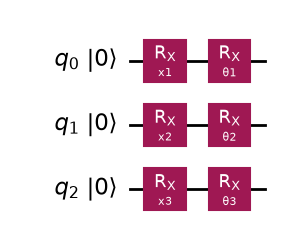
\includegraphics[width=0.3\textwidth]{figures/hidden3_1.png}
\caption[short]{First hidden layer of rotation gates}
\label{fig:hidden3_1}
\end{figure}

\subsection{Hidden Layer - Entanglement}
What's getting more interesting is the CNOT gate in the next layer. If we only apply rotation gates on each qubit separately, there is no interactions between qubits. CNOT gate allows interactions between qubits so that information can be passed across qubits instead of just staying at only a single qubit. A good analogy is that in classical neural networks, each neuron takes all the neurons in the previous layer as inputs, if we assume fully-connected layers.\\
Although we have a 3-qubit system, but let's look at the first two qubits $q_0,q_1$. In Figure~\ref{fig:cnot}, after encoding layer and first rotation layer, the state of each qubit is:

\begin{equation}
\begin{aligned}
\ket{q_0}=\cos(\frac{\theta_1+x_1}{2})\ket{0}+(-i\sin(\frac{\theta_1+x_1}{2}))\ket{1}\\
\ket{q_1}= \cos(\frac{\theta_2+x_2}{2})\ket{0}+(-i\sin(\frac{\theta_2+x_2}{2}))\ket{1}
\end{aligned}    
\end{equation}


\begin{figure}[htbp]
    \centering
    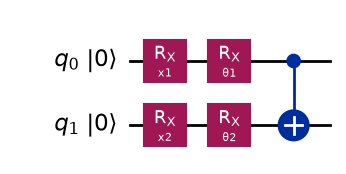
\includegraphics[width=0.3\textwidth]{figures/cnot.png}
    \caption[short]{CNOT gate layer on two qubits after rotation gates}
    \label{fig:cnot}
\end{figure}

The state of entire system is:
\begin{equation}
\ket{q_1q_0}=
\begin{bmatrix}
    \cos(\frac{\theta_1+x_1}{2})\cos(\frac{\theta_2+x_2}{2})\\
    -i\cos(\frac{\theta_2+x_2}{2})\sin(\frac{\theta_1+x_1}{2})\\
    -i\cos(\frac{\theta_1+x_1}{2})\sin(\frac{\theta_2+x_2}{2})\\
    -\sin(\frac{\theta_1+x_1}{2})\sin(\frac{\theta_2+x_2}{2})
\end{bmatrix}
\label{eq:stateof2}
\end{equation}

If we apply a CNOT gate on these two qubits, then we have:
\begin{equation}
    CNOT\ket{q_1q_0}=\begin{bmatrix}1&0&0&0\\0&0&0&1\\0&0&1&0\\0&1&0&0\end{bmatrix}\times 
    \begin{bmatrix}
    \cos(\frac{\theta_1+x_1}{2})\cos(\frac{\theta_2+x_2}{2})\\
    -i\cos(\frac{\theta_2+x_2}{2})\sin(\frac{\theta_1+x_1}{2})\\
    -i\cos(\frac{\theta_1+x_1}{2})\sin(\frac{\theta_2+x_2}{2})\\
    -\sin(\frac{\theta_1+x_1}{2})\sin(\frac{\theta_2+x_2}{2})
\end{bmatrix}=\begin{bmatrix}
    \cos(\frac{\theta_1+x_1}{2})\cos(\frac{\theta_2+x_2}{2})\\
    -\sin(\frac{\theta_1+x_1}{2})\sin(\frac{\theta_2+x_2}{2})\\
    -i\cos(\frac{\theta_1+x_1}{2})\sin(\frac{\theta_2+x_2}{2})\\
    -i\cos(\frac{\theta_2+x_2}{2})\sin(\frac{\theta_1+x_1}{2})
\end{bmatrix}
\label{eq:cnoton2}
\end{equation}
As you might observe, the second element and the fourth element of state vector got swapped. Now, these two qubits are entangled! This means that the system cannot be rewriten into a tensor product of two single qubit anymore. You can easily verify this by yourself using Eq.~\ref{eq:entangle}. 
\begin{equation*}
    CNOT\ket{q_1q_0}\neq \ket{q_1}\otimes\ket{q_0}
\end{equation*}
Now, if take the third qubit into consideration and look at the entire system, the operation matrix is:
\begin{equation}
\begin{aligned}
U_{entangle} = I\otimes CNOT_{q_0\rightarrow q_1}
\end{aligned}
\end{equation}
where $I$ is $2\times2$ identity matrix. To expand, we have
\begin{equation}
\begin{aligned}
U_{entangle} &= \begin{bmatrix}1&0\\0&1\end{bmatrix}\otimes\begin{bmatrix}1&0&0&0\\0&0&0&1\\0&0&1&0\\0&1&0&0\end{bmatrix}\\
&=\begin{bmatrix}
1&0&0&0&0&0&0&0\\0&0&0&1&0&0&0&0\\0&0&1&0&0&0&0&0\\0&1&0&0&0&0&0&0\\
0&0&0&0&1&0&0&0\\0&0&0&0&0&0&0&1\\0&0&0&0&0&0&1&0\\0&0&0&0&0&1&0&0
\end{bmatrix}
\end{aligned}
\label{eq:entanglematrix}
\end{equation}

\begin{figure}[htbp]
    \centering
    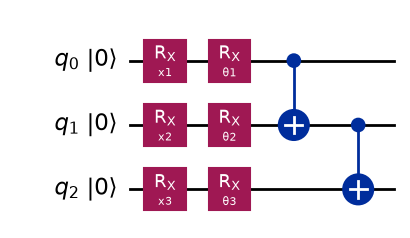
\includegraphics[width=0.3\textwidth]{figures/entangle3.png}
    \caption[short]{Entanglement layer in QNN}
    \label{fig:entangle3}
\end{figure}

Then, we can apply this matrix~\ref{eq:entanglematrix} on the statevector we derived from Eq~\ref{eq:statevector-hidden1}:
\begin{equation}
\begin{aligned}
\begin{bmatrix}1&0&0&0&0&0&0&0\\0&0&0&1&0&0&0&0\\0&0&1&0&0&0&0&0\\0&1&0&0&0&0&0&0\\
0&0&0&0&1&0&0&0\\0&0&0&0&0&0&0&1\\0&0&0&0&0&0&1&0\\0&0&0&0&0&1&0&0\end{bmatrix}\times
\begin{bmatrix}
\cos(\frac{\theta_3+x_3}{2})\cos(\frac{\theta_2+x_2}{2})\cos(\frac{\theta_1+x_1}{2})\\[6pt]
-i\cos(\frac{\theta_3+x_3}{2})\cos(\frac{\theta_2+x_2}{2})\sin(\frac{\theta_1+x_1}{2})\\[6pt]
-i\cos(\frac{\theta_3+x_3}{2})\sin(\frac{\theta_2+x_2}{2})\cos(\frac{\theta_1+x_1}{2})\\[6pt]
-\cos(\frac{\theta_3+x_3}{2})\sin(\frac{\theta_2+x_2}{2})\sin(\frac{\theta_1+x_1}{2})\\[6pt]
-i\sin(\frac{\theta_3+x_3}{2})\cos(\frac{\theta_2+x_2}{2})\cos(\frac{\theta_1+x_1}{2})\\[6pt]
-\sin(\frac{\theta_3+x_3}{2})\cos(\frac{\theta_2+x_2}{2})\sin(\frac{\theta_1+x_1}{2})\\[6pt]
-\sin(\frac{\theta_3+x_3}{2})\sin(\frac{\theta_2+x_2}{2})\cos(\frac{\theta_1+x_1}{2})\\[6pt]
i\sin(\frac{\theta_3+x_3}{2})\sin(\frac{\theta_2+x_2}{2})\sin(\frac{\theta_1+x_1}{2})
\end{bmatrix}=
\begin{bmatrix}
\cos(\frac{\theta_3+x_3}{2})\cos(\frac{\theta_2+x_2}{2})\cos(\frac{\theta_1+x_1}{2})\\[6pt]
-\cos(\frac{\theta_3+x_3}{2})\sin(\frac{\theta_2+x_2}{2})\sin(\frac{\theta_1+x_1}{2})\\[6pt]
-i\cos(\frac{\theta_3+x_3}{2})\sin(\frac{\theta_2+x_2}{2})\cos(\frac{\theta_1+x_1}{2})\\[6pt]
-i\cos(\frac{\theta_3+x_3}{2})\cos(\frac{\theta_2+x_2}{2})\sin(\frac{\theta_1+x_1}{2})\\[6pt]
-i\sin(\frac{\theta_3+x_3}{2})\cos(\frac{\theta_2+x_2}{2})\cos(\frac{\theta_1+x_1}{2})\\[6pt]
i\sin(\frac{\theta_3+x_3}{2})\sin(\frac{\theta_2+x_2}{2})\sin(\frac{\theta_1+x_1}{2})\\[6pt]
-\sin(\frac{\theta_3+x_3}{2})\sin(\frac{\theta_2+x_2}{2})\cos(\frac{\theta_1+x_1}{2})\\[6pt]
-\sin(\frac{\theta_3+x_3}{2})\cos(\frac{\theta_2+x_2}{2})\sin(\frac{\theta_1+x_1}{2})
\end{bmatrix}    
\end{aligned}
\label{eq:cnot1}
\end{equation}
Please notice that the original order $(1,2,3,4,\quad5,6,7,8)$ becomes $(1,4,3,2,\quad 5,8,7,6)$. For every ``subgroup'', the second and fourth element are swapped. \\
Then, as Figure~\ref{fig:entangle3} shows, we apply CNOT gate on the second and third qubits $q_1,q_2$, the operation matrix is:
\begin{equation*}
\begin{aligned}
U_{entangle}&=CNOT_{q_1\rightarrow q_2}\otimes I\\
&=\begin{bmatrix}1&0&0&0\\0&0&0&1\\0&0&1&0\\0&1&0&0\end{bmatrix}\otimes\begin{bmatrix}1&0\\0&1\end{bmatrix}
&=\begin{bmatrix}1&0&0&0&0&0&0&0\\0&1&0&0&0&0&0&0\\0&0&0&0&0&0&1&0\\0&0&0&0&0&0&0&1\\
0&0&0&0&1&0&0&0\\0&0&0&0&0&1&0&0\\0&0&1&0&0&0&0&0\\0&0&0&1&0&0&0&0\end{bmatrix}
\end{aligned}
\end{equation*}
Then, we apply this matrix on  the statevector:
\begin{equation*}
\begin{bmatrix}1&0&0&0&0&0&0&0\\0&1&0&0&0&0&0&0\\0&0&0&0&0&0&1&0\\0&0&0&0&0&0&0&1\\
0&0&0&0&1&0&0&0\\0&0&0&0&0&1&0&0\\0&0&1&0&0&0&0&0\\0&0&0&1&0&0&0&0\end{bmatrix}\times
\begin{bmatrix}
\cos(\frac{\theta_3+x_3}{2})\cos(\frac{\theta_2+x_2}{2})\cos(\frac{\theta_1+x_1}{2})\\[6pt]
-\cos(\frac{\theta_3+x_3}{2})\sin(\frac{\theta_2+x_2}{2})\sin(\frac{\theta_1+x_1}{2})\\[6pt]
-i\cos(\frac{\theta_3+x_3}{2})\sin(\frac{\theta_2+x_2}{2})\cos(\frac{\theta_1+x_1}{2})\\[6pt]
-i\cos(\frac{\theta_3+x_3}{2})\cos(\frac{\theta_2+x_2}{2})\sin(\frac{\theta_1+x_1}{2})\\[6pt]
-i\sin(\frac{\theta_3+x_3}{2})\cos(\frac{\theta_2+x_2}{2})\cos(\frac{\theta_1+x_1}{2})\\[6pt]
i\sin(\frac{\theta_3+x_3}{2})\sin(\frac{\theta_2+x_2}{2})\sin(\frac{\theta_1+x_1}{2})\\[6pt]
-\sin(\frac{\theta_3+x_3}{2})\sin(\frac{\theta_2+x_2}{2})\cos(\frac{\theta_1+x_1}{2})\\[6pt]
-\sin(\frac{\theta_3+x_3}{2})\cos(\frac{\theta_2+x_2}{2})\sin(\frac{\theta_1+x_1}{2})
\end{bmatrix}=\begin{bmatrix}
\cos(\frac{\theta_3+x_3}{2})\cos(\frac{\theta_2+x_2}{2})\cos(\frac{\theta_1+x_1}{2})\\[6pt]
-\cos(\frac{\theta_3+x_3}{2})\sin(\frac{\theta_2+x_2}{2})\sin(\frac{\theta_1+x_1}{2})\\[6pt]
-\sin(\frac{\theta_3+x_3}{2})\sin(\frac{\theta_2+x_2}{2})\cos(\frac{\theta_1+x_1}{2})\\[6pt]
-\sin(\frac{\theta_3+x_3}{2})\cos(\frac{\theta_2+x_2}{2})\sin(\frac{\theta_1+x_1}{2})\\[6pt]
-i\sin(\frac{\theta_3+x_3}{2})\cos(\frac{\theta_2+x_2}{2})\cos(\frac{\theta_1+x_1}{2})\\[6pt]
i\sin(\frac{\theta_3+x_3}{2})\sin(\frac{\theta_2+x_2}{2})\sin(\frac{\theta_1+x_1}{2})\\[6pt]
-i\cos(\frac{\theta_3+x_3}{2})\sin(\frac{\theta_2+x_2}{2})\cos(\frac{\theta_1+x_1}{2})\\[6pt]
-i\cos(\frac{\theta_3+x_3}{2})\cos(\frac{\theta_2+x_2}{2})\sin(\frac{\theta_1+x_1}{2})
\end{bmatrix}
\end{equation*}
If you look carefully, What happens is that compare with Eq.~\ref{eq:cnot1}, swapping happens as follows:
\begin{equation*}
    3\leftrightarrow7,\quad 4\leftrightarrow8
\end{equation*}
As you might observe, you can apply a CNOT gate on any of the two qubits (e.g., $q_0,q_2$) and CNOT gates are essentially just permutation matrix that induces a permutation of amplitude in statevector. The magic is that all these four qubits are entangled meaning the statevector is not simply a tensor product of four single-qubit statevector:
\begin{equation*}
    \ket{q_2q_1q_0}\neq\ket{q_2}\otimes\ket{q_1}\otimes\ket{q_0}
\end{equation*}
\subsection{Information Propogation through CNOT Gates}
The importance of CNOT gate is allowing information be propogatied from control qubit to target qubit, if we measure in Z-basis. Let's look at a 2-qubit system first. Previously, we have derived states of 2-qubit system in Eq.~\ref{eq:stateof2} that after a layer of encoding and rotation. The probability of observing $q_1=0$ is as follows. 
\begin{equation}
\begin{aligned}
\text{Let}\quad \alpha&=\frac{x_1+\theta_1}{2},\quad \beta=\frac{x_2+\theta_2}{2}\\
P(\ket{q_1}=\ket{0})&=\cos^2(\alpha)\cos^2(\beta)+\cos^2(\beta)\sin^2(\alpha)\\
&=\cos^2(\beta)(\cos^2(\alpha)+\sin^2(\alpha))\\
&=\cos^2(\beta)=\cos(\frac{x_2+\theta_2}{2})
\end{aligned}
\end{equation}
As you can see, the probability of each state in $q_1$ is a function of $x2$ and $\theta_2$:
\begin{equation*}
    P(\ket{q_1}=\ket{0})=f(x_2,\theta_2)
\end{equation*}
However, after a CNOT gate, the statevector becomes Eq.~\ref{eq:cnoton2}. The The probability of observing $q_1=0$ becomes as follwoing. 
\begin{equation}
\begin{aligned}
P(\ket{q_1}=\ket{0})&=\cos^2(\alpha)\cos^2(\alpha)+\sin^2(\alpha)\sin^2(\beta)\\
&=\cos^2(\frac{x_1+\theta_1}{2})\cos^2(\frac{x_2+\theta_2}{2})+\sin^2(\frac{x_1+\theta_1}{2})\sin^2(\frac{x_2+\theta_2}{2})\\
&=f(x_1,x_2,\theta_1,\theta_2)
\end{aligned}
\end{equation}
Now, as you can see, the probability amplitude of $q_1$ becomes a function of $x_1,x_2,\theta_1,\theta_2$! The information from $q_0$, the first qubit, both input value $x_1$ and parameters $\theta_1$ are passed down to $q_1$. This gives the circuits much greater expressivity. However, another thing to notice is that the probability of $q_0$ does not change before or after CNOT gate. 
\begin{equation}
    P(\ket{q_0}=\ket{0})=\cos^2(\frac{\theta_1+x_1}{2})
\end{equation}
Intrestingly, the infomration did not pass from target to control. However, this is given we measure in Z-basis. Measurement in other basis will lead to different sitautions.\\
Again, if we compare with classical neural networks, it's a function of all the input values as Eq.~\ref{eq:nnfunc} shows. This is also knonw as fully connected layers. If the output of a classical Nueral Networks is function of only a single input $x_i$, it will not be able learn the latent structure of the data, significantly harming the expressivity. The entanglement layer tries to do the similar thing. 
\begin{equation}
\begin{aligned}
f_{NN}&=f(\sigma(W^TX+b))\\
&=f(\sigma(\sum_{n=1}^{N}w_nx_n+b))\\
&=f(x_1,x_2,\cdots,x_N,W)
\end{aligned}
\label{eq:nnfunc}
\end{equation}
Now, let's look at the 3-qubit system. Before the entanglment layer, the probability of observing the fourth qubit $\ket{q_3}=\ket{0}$ can be derived from Eq.~\ref{eq:statevector-hidden1} as follows:




\end{document}